\documentclass[twoside]{book}

% Packages required by doxygen
\usepackage{fixltx2e}
\usepackage{calc}
\usepackage{doxygen}
\usepackage[export]{adjustbox} % also loads graphicx
\usepackage{graphicx}
\usepackage[utf8]{inputenc}
\usepackage{makeidx}
\usepackage{multicol}
\usepackage{multirow}
\PassOptionsToPackage{warn}{textcomp}
\usepackage{textcomp}
\usepackage[nointegrals]{wasysym}
\usepackage[table]{xcolor}

% Font selection
\usepackage[T1]{fontenc}
\usepackage[scaled=.90]{helvet}
\usepackage{courier}
\usepackage{amssymb}
\usepackage{sectsty}
\renewcommand{\familydefault}{\sfdefault}
\allsectionsfont{%
  \fontseries{bc}\selectfont%
  \color{darkgray}%
}
\renewcommand{\DoxyLabelFont}{%
  \fontseries{bc}\selectfont%
  \color{darkgray}%
}
\newcommand{\+}{\discretionary{\mbox{\scriptsize$\hookleftarrow$}}{}{}}

% Page & text layout
\usepackage{geometry}
\geometry{%
  a4paper,%
  top=2.5cm,%
  bottom=2.5cm,%
  left=2.5cm,%
  right=2.5cm%
}
\tolerance=750
\hfuzz=15pt
\hbadness=750
\setlength{\emergencystretch}{15pt}
\setlength{\parindent}{0cm}
\setlength{\parskip}{3ex plus 2ex minus 2ex}
\makeatletter
\renewcommand{\paragraph}{%
  \@startsection{paragraph}{4}{0ex}{-1.0ex}{1.0ex}{%
    \normalfont\normalsize\bfseries\SS@parafont%
  }%
}
\renewcommand{\subparagraph}{%
  \@startsection{subparagraph}{5}{0ex}{-1.0ex}{1.0ex}{%
    \normalfont\normalsize\bfseries\SS@subparafont%
  }%
}
\makeatother

% Headers & footers
\usepackage{fancyhdr}
\pagestyle{fancyplain}
\fancyhead[LE]{\fancyplain{}{\bfseries\thepage}}
\fancyhead[CE]{\fancyplain{}{}}
\fancyhead[RE]{\fancyplain{}{\bfseries\leftmark}}
\fancyhead[LO]{\fancyplain{}{\bfseries\rightmark}}
\fancyhead[CO]{\fancyplain{}{}}
\fancyhead[RO]{\fancyplain{}{\bfseries\thepage}}
\fancyfoot[LE]{\fancyplain{}{}}
\fancyfoot[CE]{\fancyplain{}{}}
\fancyfoot[RE]{\fancyplain{}{\bfseries\scriptsize Generated by Doxygen }}
\fancyfoot[LO]{\fancyplain{}{\bfseries\scriptsize Generated by Doxygen }}
\fancyfoot[CO]{\fancyplain{}{}}
\fancyfoot[RO]{\fancyplain{}{}}
\renewcommand{\footrulewidth}{0.4pt}
\renewcommand{\chaptermark}[1]{%
  \markboth{#1}{}%
}
\renewcommand{\sectionmark}[1]{%
  \markright{\thesection\ #1}%
}

% Indices & bibliography
\usepackage{natbib}
\usepackage[titles]{tocloft}
\setcounter{tocdepth}{3}
\setcounter{secnumdepth}{5}
\makeindex

% Hyperlinks (required, but should be loaded last)
\usepackage{ifpdf}
\ifpdf
  \usepackage[pdftex,pagebackref=true]{hyperref}
\else
  \usepackage[ps2pdf,pagebackref=true]{hyperref}
\fi
\hypersetup{%
  colorlinks=true,%
  linkcolor=blue,%
  citecolor=blue,%
  unicode%
}

% Custom commands
\newcommand{\clearemptydoublepage}{%
  \newpage{\pagestyle{empty}\cleardoublepage}%
}

\usepackage{caption}
\captionsetup{labelsep=space,justification=centering,font={bf},singlelinecheck=off,skip=4pt,position=top}

%===== C O N T E N T S =====

\begin{document}

% Titlepage & ToC
\hypersetup{pageanchor=false,
             bookmarksnumbered=true,
             pdfencoding=unicode
            }
\pagenumbering{roman}
\begin{titlepage}
\vspace*{7cm}
\begin{center}%
{\Large My Project }\\
\vspace*{1cm}
{\large Generated by Doxygen 1.8.11}\\
\end{center}
\end{titlepage}
\clearemptydoublepage
\tableofcontents
\clearemptydoublepage
\pagenumbering{arabic}
\hypersetup{pageanchor=true}

%--- Begin generated contents ---
\chapter{Class Index}
\section{Class List}
Here are the classes, structs, unions and interfaces with brief descriptions\+:\begin{DoxyCompactList}
\item\contentsline{section}{\hyperlink{structnode}{node} }{\pageref{structnode}}{}
\item\contentsline{section}{\hyperlink{structnode1}{node1} }{\pageref{structnode1}}{}
\item\contentsline{section}{\hyperlink{structnode__info}{node\+\_\+info} }{\pageref{structnode__info}}{}
\end{DoxyCompactList}

\chapter{File Index}
\section{File List}
Here is a list of all files with brief descriptions\+:\begin{DoxyCompactList}
\item\contentsline{section}{\hyperlink{Lab1_8c}{Lab1.\+c} }{\pageref{Lab1_8c}}{}
\end{DoxyCompactList}

\chapter{Class Documentation}
\hypertarget{classComplex}{}\section{Complex Class Reference}
\label{classComplex}\index{Complex@{Complex}}


{\ttfamily \#include $<$Complex.\+h$>$}

\subsection*{Public Member Functions}
\begin{DoxyCompactItemize}
\item 
\hyperlink{classComplex_a2bce7c231cd74634e24deb37b4e2d61d}{Complex} (double \hyperlink{classComplex_a0138f5fe2b2c6180b8fcda77a7aa51c5}{real}=0.\+0, double \hyperlink{classComplex_a2bb90cc563599c3c8bdec9acf9ea40a6}{imag}=0.\+0)
\item 
double \hyperlink{classComplex_abe3d69aff637b06e1c1f73c14368d77d}{get\+Real} () const 
\item 
void \hyperlink{classComplex_ac767331bf173de715f47589d6f614a6d}{set\+Real} (double \hyperlink{classComplex_a0138f5fe2b2c6180b8fcda77a7aa51c5}{real})
\item 
double \hyperlink{classComplex_a06791ae9b7d850ef7de11d93e997af94}{get\+Imag} () const 
\item 
void \hyperlink{classComplex_ab94d5256ccb9a936df00e4bdd6f8f259}{set\+Imag} (double \hyperlink{classComplex_a2bb90cc563599c3c8bdec9acf9ea40a6}{imag})
\item 
void \hyperlink{classComplex_a753e3d6a1b2df1950ba4caebe70382fe}{set\+Value} (double \hyperlink{classComplex_a0138f5fe2b2c6180b8fcda77a7aa51c5}{real}, double \hyperlink{classComplex_a2bb90cc563599c3c8bdec9acf9ea40a6}{imag})
\item 
void \hyperlink{classComplex_a7c2092a00caf353537f698316be20b19}{print} () const 
\item 
bool \hyperlink{classComplex_a5775caffefa608486555f2bdac89a1ec}{is\+Real} () const 
\item 
bool \hyperlink{classComplex_ace89217819bbbd46a9a9f2e51ea7beed}{is\+Imaginary} () const 
\item 
\hyperlink{classComplex}{Complex} \& \hyperlink{classComplex_aa6e77da8ab7b7177b12a7fb0c4fb9e75}{add\+Into} (const \hyperlink{classComplex}{Complex} \&another)
\item 
\hyperlink{classComplex}{Complex} \& \hyperlink{classComplex_ad0a009826e3f2b972c5a4dbf40bd3805}{add\+Into} (double \hyperlink{classComplex_a0138f5fe2b2c6180b8fcda77a7aa51c5}{real}, double \hyperlink{classComplex_a2bb90cc563599c3c8bdec9acf9ea40a6}{imag})
\item 
\hyperlink{classComplex}{Complex} \hyperlink{classComplex_a9461ded91a8b436b6c01a0549a7982e3}{add\+Return\+New} (const \hyperlink{classComplex}{Complex} \&another) const 
\item 
\hyperlink{classComplex}{Complex} \hyperlink{classComplex_a2e9ef45e71d07776d7cbd4999d6d85a7}{add\+Return\+New} (double \hyperlink{classComplex_a0138f5fe2b2c6180b8fcda77a7aa51c5}{real}, double \hyperlink{classComplex_a2bb90cc563599c3c8bdec9acf9ea40a6}{imag}) const 
\end{DoxyCompactItemize}
\subsection*{Private Attributes}
\begin{DoxyCompactItemize}
\item 
double \hyperlink{classComplex_a0138f5fe2b2c6180b8fcda77a7aa51c5}{real}
\item 
double \hyperlink{classComplex_a2bb90cc563599c3c8bdec9acf9ea40a6}{imag}
\end{DoxyCompactItemize}


\subsection{Constructor \& Destructor Documentation}
\index{Complex@{Complex}!Complex@{Complex}}
\index{Complex@{Complex}!Complex@{Complex}}
\subsubsection[{\texorpdfstring{Complex(double real=0.\+0, double imag=0.\+0)}{Complex(double real=0.0, double imag=0.0)}}]{\setlength{\rightskip}{0pt plus 5cm}Complex\+::\+Complex (
\begin{DoxyParamCaption}
\item[{double}]{real = {\ttfamily 0.0}, }
\item[{double}]{imag = {\ttfamily 0.0}}
\end{DoxyParamCaption}
)}\hypertarget{classComplex_a2bce7c231cd74634e24deb37b4e2d61d}{}\label{classComplex_a2bce7c231cd74634e24deb37b4e2d61d}

\begin{DoxyCode}
7    : \hyperlink{classComplex_a0138f5fe2b2c6180b8fcda77a7aa51c5}{real}(\hyperlink{classComplex_a0138f5fe2b2c6180b8fcda77a7aa51c5}{real}), \hyperlink{classComplex_a2bb90cc563599c3c8bdec9acf9ea40a6}{imag}(\hyperlink{classComplex_a2bb90cc563599c3c8bdec9acf9ea40a6}{imag}) \{ \}
\end{DoxyCode}


\subsection{Member Function Documentation}
\index{Complex@{Complex}!add\+Into@{add\+Into}}
\index{add\+Into@{add\+Into}!Complex@{Complex}}
\subsubsection[{\texorpdfstring{add\+Into(const Complex \&another)}{addInto(const Complex &another)}}]{\setlength{\rightskip}{0pt plus 5cm}{\bf Complex} \& Complex\+::add\+Into (
\begin{DoxyParamCaption}
\item[{const {\bf Complex} \&}]{another}
\end{DoxyParamCaption}
)}\hypertarget{classComplex_aa6e77da8ab7b7177b12a7fb0c4fb9e75}{}\label{classComplex_aa6e77da8ab7b7177b12a7fb0c4fb9e75}

\begin{DoxyCode}
45                                                   \{
46    \hyperlink{classComplex_a0138f5fe2b2c6180b8fcda77a7aa51c5}{real} += another.\hyperlink{classComplex_a0138f5fe2b2c6180b8fcda77a7aa51c5}{real};
47    \hyperlink{classComplex_a2bb90cc563599c3c8bdec9acf9ea40a6}{imag} += another.\hyperlink{classComplex_a2bb90cc563599c3c8bdec9acf9ea40a6}{imag};
48    \textcolor{keywordflow}{return} *\textcolor{keyword}{this};
49 \}
\end{DoxyCode}
\index{Complex@{Complex}!add\+Into@{add\+Into}}
\index{add\+Into@{add\+Into}!Complex@{Complex}}
\subsubsection[{\texorpdfstring{add\+Into(double real, double imag)}{addInto(double real, double imag)}}]{\setlength{\rightskip}{0pt plus 5cm}{\bf Complex} \& Complex\+::add\+Into (
\begin{DoxyParamCaption}
\item[{double}]{real, }
\item[{double}]{imag}
\end{DoxyParamCaption}
)}\hypertarget{classComplex_ad0a009826e3f2b972c5a4dbf40bd3805}{}\label{classComplex_ad0a009826e3f2b972c5a4dbf40bd3805}

\begin{DoxyCode}
51                                                    \{
52    this->\hyperlink{classComplex_a0138f5fe2b2c6180b8fcda77a7aa51c5}{real} += \hyperlink{classComplex_a0138f5fe2b2c6180b8fcda77a7aa51c5}{real};
53    this->\hyperlink{classComplex_a2bb90cc563599c3c8bdec9acf9ea40a6}{imag} += \hyperlink{classComplex_a2bb90cc563599c3c8bdec9acf9ea40a6}{imag};
54    \textcolor{keywordflow}{return} *\textcolor{keyword}{this};
55 \}
\end{DoxyCode}
\index{Complex@{Complex}!add\+Return\+New@{add\+Return\+New}}
\index{add\+Return\+New@{add\+Return\+New}!Complex@{Complex}}
\subsubsection[{\texorpdfstring{add\+Return\+New(const Complex \&another) const }{addReturnNew(const Complex &another) const }}]{\setlength{\rightskip}{0pt plus 5cm}{\bf Complex} Complex\+::add\+Return\+New (
\begin{DoxyParamCaption}
\item[{const {\bf Complex} \&}]{another}
\end{DoxyParamCaption}
) const}\hypertarget{classComplex_a9461ded91a8b436b6c01a0549a7982e3}{}\label{classComplex_a9461ded91a8b436b6c01a0549a7982e3}

\begin{DoxyCode}
58                                                            \{
59    \textcolor{keywordflow}{return} \hyperlink{classComplex_a2bce7c231cd74634e24deb37b4e2d61d}{Complex}(\hyperlink{classComplex_a0138f5fe2b2c6180b8fcda77a7aa51c5}{real} + another.\hyperlink{classComplex_a0138f5fe2b2c6180b8fcda77a7aa51c5}{real}, \hyperlink{classComplex_a2bb90cc563599c3c8bdec9acf9ea40a6}{imag} + another.\hyperlink{classComplex_a2bb90cc563599c3c8bdec9acf9ea40a6}{imag});
60 \}
\end{DoxyCode}


Here is the call graph for this function\+:
\nopagebreak
\begin{figure}[H]
\begin{center}
\leavevmode
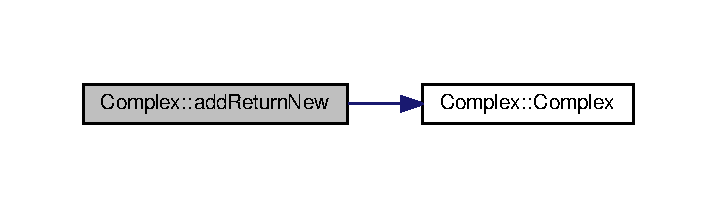
\includegraphics[width=344pt]{classComplex_a9461ded91a8b436b6c01a0549a7982e3_cgraph}
\end{center}
\end{figure}


\index{Complex@{Complex}!add\+Return\+New@{add\+Return\+New}}
\index{add\+Return\+New@{add\+Return\+New}!Complex@{Complex}}
\subsubsection[{\texorpdfstring{add\+Return\+New(double real, double imag) const }{addReturnNew(double real, double imag) const }}]{\setlength{\rightskip}{0pt plus 5cm}{\bf Complex} Complex\+::add\+Return\+New (
\begin{DoxyParamCaption}
\item[{double}]{real, }
\item[{double}]{imag}
\end{DoxyParamCaption}
) const}\hypertarget{classComplex_a2e9ef45e71d07776d7cbd4999d6d85a7}{}\label{classComplex_a2e9ef45e71d07776d7cbd4999d6d85a7}

\begin{DoxyCode}
62                                                             \{
63    \textcolor{keywordflow}{return} \hyperlink{classComplex_a2bce7c231cd74634e24deb37b4e2d61d}{Complex}(this->\hyperlink{classComplex_a0138f5fe2b2c6180b8fcda77a7aa51c5}{real} + \hyperlink{classComplex_a0138f5fe2b2c6180b8fcda77a7aa51c5}{real}, this->\hyperlink{classComplex_a2bb90cc563599c3c8bdec9acf9ea40a6}{imag} + \hyperlink{classComplex_a2bb90cc563599c3c8bdec9acf9ea40a6}{imag});
64 \}\end{DoxyCode}


Here is the call graph for this function\+:
\nopagebreak
\begin{figure}[H]
\begin{center}
\leavevmode
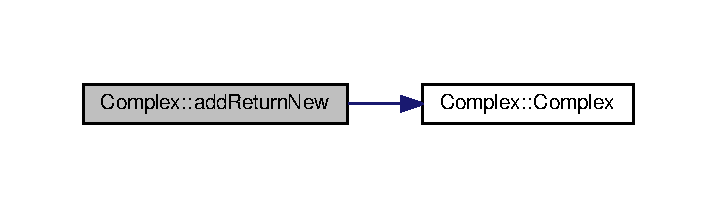
\includegraphics[width=344pt]{classComplex_a2e9ef45e71d07776d7cbd4999d6d85a7_cgraph}
\end{center}
\end{figure}


\index{Complex@{Complex}!get\+Imag@{get\+Imag}}
\index{get\+Imag@{get\+Imag}!Complex@{Complex}}
\subsubsection[{\texorpdfstring{get\+Imag() const }{getImag() const }}]{\setlength{\rightskip}{0pt plus 5cm}double Complex\+::get\+Imag (
\begin{DoxyParamCaption}
{}
\end{DoxyParamCaption}
) const}\hypertarget{classComplex_a06791ae9b7d850ef7de11d93e997af94}{}\label{classComplex_a06791ae9b7d850ef7de11d93e997af94}

\begin{DoxyCode}
17                               \{
18    \textcolor{keywordflow}{return} \hyperlink{classComplex_a2bb90cc563599c3c8bdec9acf9ea40a6}{imag};
19 \}
\end{DoxyCode}
\index{Complex@{Complex}!get\+Real@{get\+Real}}
\index{get\+Real@{get\+Real}!Complex@{Complex}}
\subsubsection[{\texorpdfstring{get\+Real() const }{getReal() const }}]{\setlength{\rightskip}{0pt plus 5cm}double Complex\+::get\+Real (
\begin{DoxyParamCaption}
{}
\end{DoxyParamCaption}
) const}\hypertarget{classComplex_abe3d69aff637b06e1c1f73c14368d77d}{}\label{classComplex_abe3d69aff637b06e1c1f73c14368d77d}

\begin{DoxyCode}
9                               \{
10    \textcolor{keywordflow}{return} \hyperlink{classComplex_a0138f5fe2b2c6180b8fcda77a7aa51c5}{real};
11 \}
\end{DoxyCode}
\index{Complex@{Complex}!is\+Imaginary@{is\+Imaginary}}
\index{is\+Imaginary@{is\+Imaginary}!Complex@{Complex}}
\subsubsection[{\texorpdfstring{is\+Imaginary() const }{isImaginary() const }}]{\setlength{\rightskip}{0pt plus 5cm}bool Complex\+::is\+Imaginary (
\begin{DoxyParamCaption}
{}
\end{DoxyParamCaption}
) const}\hypertarget{classComplex_ace89217819bbbd46a9a9f2e51ea7beed}{}\label{classComplex_ace89217819bbbd46a9a9f2e51ea7beed}

\begin{DoxyCode}
39                                 \{
40    \textcolor{keywordflow}{return} (\hyperlink{classComplex_a0138f5fe2b2c6180b8fcda77a7aa51c5}{real} == 0);
41 \}
\end{DoxyCode}
\index{Complex@{Complex}!is\+Real@{is\+Real}}
\index{is\+Real@{is\+Real}!Complex@{Complex}}
\subsubsection[{\texorpdfstring{is\+Real() const }{isReal() const }}]{\setlength{\rightskip}{0pt plus 5cm}bool Complex\+::is\+Real (
\begin{DoxyParamCaption}
{}
\end{DoxyParamCaption}
) const}\hypertarget{classComplex_a5775caffefa608486555f2bdac89a1ec}{}\label{classComplex_a5775caffefa608486555f2bdac89a1ec}

\begin{DoxyCode}
35                            \{
36    \textcolor{keywordflow}{return} (\hyperlink{classComplex_a2bb90cc563599c3c8bdec9acf9ea40a6}{imag} == 0);
37 \}
\end{DoxyCode}
\index{Complex@{Complex}!print@{print}}
\index{print@{print}!Complex@{Complex}}
\subsubsection[{\texorpdfstring{print() const }{print() const }}]{\setlength{\rightskip}{0pt plus 5cm}void Complex\+::print (
\begin{DoxyParamCaption}
{}
\end{DoxyParamCaption}
) const}\hypertarget{classComplex_a7c2092a00caf353537f698316be20b19}{}\label{classComplex_a7c2092a00caf353537f698316be20b19}

\begin{DoxyCode}
31                           \{
32    cout << \textcolor{charliteral}{'('} << \hyperlink{classComplex_a0138f5fe2b2c6180b8fcda77a7aa51c5}{real} << \textcolor{charliteral}{','} << \hyperlink{classComplex_a2bb90cc563599c3c8bdec9acf9ea40a6}{imag} << \textcolor{charliteral}{')'} << endl;
33 \}
\end{DoxyCode}
\index{Complex@{Complex}!set\+Imag@{set\+Imag}}
\index{set\+Imag@{set\+Imag}!Complex@{Complex}}
\subsubsection[{\texorpdfstring{set\+Imag(double imag)}{setImag(double imag)}}]{\setlength{\rightskip}{0pt plus 5cm}void Complex\+::set\+Imag (
\begin{DoxyParamCaption}
\item[{double}]{imag}
\end{DoxyParamCaption}
)}\hypertarget{classComplex_ab94d5256ccb9a936df00e4bdd6f8f259}{}\label{classComplex_ab94d5256ccb9a936df00e4bdd6f8f259}

\begin{DoxyCode}
21                                  \{
22    this->\hyperlink{classComplex_a2bb90cc563599c3c8bdec9acf9ea40a6}{imag} = \hyperlink{classComplex_a2bb90cc563599c3c8bdec9acf9ea40a6}{imag};
23 \}
\end{DoxyCode}
\index{Complex@{Complex}!set\+Real@{set\+Real}}
\index{set\+Real@{set\+Real}!Complex@{Complex}}
\subsubsection[{\texorpdfstring{set\+Real(double real)}{setReal(double real)}}]{\setlength{\rightskip}{0pt plus 5cm}void Complex\+::set\+Real (
\begin{DoxyParamCaption}
\item[{double}]{real}
\end{DoxyParamCaption}
)}\hypertarget{classComplex_ac767331bf173de715f47589d6f614a6d}{}\label{classComplex_ac767331bf173de715f47589d6f614a6d}

\begin{DoxyCode}
13                                  \{
14    this->\hyperlink{classComplex_a0138f5fe2b2c6180b8fcda77a7aa51c5}{real} = \hyperlink{classComplex_a0138f5fe2b2c6180b8fcda77a7aa51c5}{real};
15 \}
\end{DoxyCode}
\index{Complex@{Complex}!set\+Value@{set\+Value}}
\index{set\+Value@{set\+Value}!Complex@{Complex}}
\subsubsection[{\texorpdfstring{set\+Value(double real, double imag)}{setValue(double real, double imag)}}]{\setlength{\rightskip}{0pt plus 5cm}void Complex\+::set\+Value (
\begin{DoxyParamCaption}
\item[{double}]{real, }
\item[{double}]{imag}
\end{DoxyParamCaption}
)}\hypertarget{classComplex_a753e3d6a1b2df1950ba4caebe70382fe}{}\label{classComplex_a753e3d6a1b2df1950ba4caebe70382fe}

\begin{DoxyCode}
25                                                \{
26    this->\hyperlink{classComplex_a0138f5fe2b2c6180b8fcda77a7aa51c5}{real} = \hyperlink{classComplex_a0138f5fe2b2c6180b8fcda77a7aa51c5}{real};
27    this->\hyperlink{classComplex_a2bb90cc563599c3c8bdec9acf9ea40a6}{imag} = \hyperlink{classComplex_a2bb90cc563599c3c8bdec9acf9ea40a6}{imag};
28 \}
\end{DoxyCode}


\subsection{Member Data Documentation}
\index{Complex@{Complex}!imag@{imag}}
\index{imag@{imag}!Complex@{Complex}}
\subsubsection[{\texorpdfstring{imag}{imag}}]{\setlength{\rightskip}{0pt plus 5cm}double Complex\+::imag\hspace{0.3cm}{\ttfamily [private]}}\hypertarget{classComplex_a2bb90cc563599c3c8bdec9acf9ea40a6}{}\label{classComplex_a2bb90cc563599c3c8bdec9acf9ea40a6}
\index{Complex@{Complex}!real@{real}}
\index{real@{real}!Complex@{Complex}}
\subsubsection[{\texorpdfstring{real}{real}}]{\setlength{\rightskip}{0pt plus 5cm}double Complex\+::real\hspace{0.3cm}{\ttfamily [private]}}\hypertarget{classComplex_a0138f5fe2b2c6180b8fcda77a7aa51c5}{}\label{classComplex_a0138f5fe2b2c6180b8fcda77a7aa51c5}


The documentation for this class was generated from the following files\+:\begin{DoxyCompactItemize}
\item 
\hyperlink{Complex_8h}{Complex.\+h}\item 
\hyperlink{Complex_8cpp}{Complex.\+cpp}\end{DoxyCompactItemize}

\chapter{File Documentation}
\hypertarget{Cmain_8cpp}{}\section{Cmain.\+cpp File Reference}
\label{Cmain_8cpp}\index{Cmain.\+cpp@{Cmain.\+cpp}}
{\ttfamily \#include $<$iostream$>$}\\*
{\ttfamily \#include $<$iomanip$>$}\\*
{\ttfamily \#include \char`\"{}Complex.\+h\char`\"{}}\\*
Include dependency graph for Cmain.\+cpp\+:
\nopagebreak
\begin{figure}[H]
\begin{center}
\leavevmode
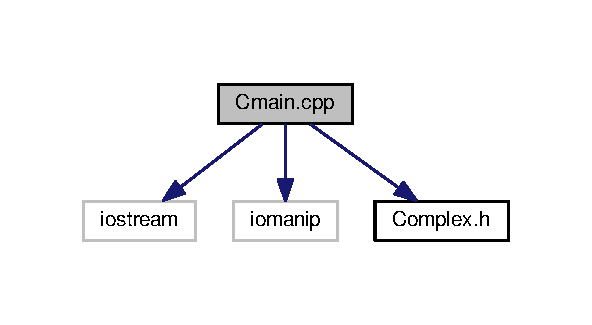
\includegraphics[width=284pt]{Cmain_8cpp__incl}
\end{center}
\end{figure}
\subsection*{Functions}
\begin{DoxyCompactItemize}
\item 
int \hyperlink{Cmain_8cpp_ae66f6b31b5ad750f1fe042a706a4e3d4}{main} ()
\end{DoxyCompactItemize}


\subsection{Function Documentation}
\index{Cmain.\+cpp@{Cmain.\+cpp}!main@{main}}
\index{main@{main}!Cmain.\+cpp@{Cmain.\+cpp}}
\subsubsection[{\texorpdfstring{main()}{main()}}]{\setlength{\rightskip}{0pt plus 5cm}int main (
\begin{DoxyParamCaption}
{}
\end{DoxyParamCaption}
)}\hypertarget{Cmain_8cpp_ae66f6b31b5ad750f1fe042a706a4e3d4}{}\label{Cmain_8cpp_ae66f6b31b5ad750f1fe042a706a4e3d4}

\begin{DoxyCode}
7            \{
8    \hyperlink{classComplex}{Complex} c1, c2(4, 5);
9    c1.\hyperlink{classComplex_a7c2092a00caf353537f698316be20b19}{print}();  \textcolor{comment}{// (0,0)}
10    c2.print();  \textcolor{comment}{// (4,5)}
11  
12    c1.\hyperlink{classComplex_a753e3d6a1b2df1950ba4caebe70382fe}{setValue}(6, 7);
13    c1.\hyperlink{classComplex_a7c2092a00caf353537f698316be20b19}{print}();  \textcolor{comment}{// (6,7)}
14  
15    c1.\hyperlink{classComplex_ac767331bf173de715f47589d6f614a6d}{setReal}(0);
16    c1.\hyperlink{classComplex_ab94d5256ccb9a936df00e4bdd6f8f259}{setImag}(8);
17    c1.\hyperlink{classComplex_a7c2092a00caf353537f698316be20b19}{print}();  \textcolor{comment}{// (0,8)}
18  
19    cout << boolalpha;  \textcolor{comment}{// print true/false instead of 0/1}
20    cout << \textcolor{stringliteral}{"Is real? "} << c1.\hyperlink{classComplex_a5775caffefa608486555f2bdac89a1ec}{isReal}() << endl;           \textcolor{comment}{// false}
21    cout << \textcolor{stringliteral}{"Is Imaginary? "} << c1.\hyperlink{classComplex_ace89217819bbbd46a9a9f2e51ea7beed}{isImaginary}() << endl; \textcolor{comment}{// true}
22  
23    c1.\hyperlink{classComplex_aa6e77da8ab7b7177b12a7fb0c4fb9e75}{addInto}(c2).\hyperlink{classComplex_aa6e77da8ab7b7177b12a7fb0c4fb9e75}{addInto}(1, 1).\hyperlink{classComplex_a7c2092a00caf353537f698316be20b19}{print}();  \textcolor{comment}{// (5,14)}
24    c1.\hyperlink{classComplex_a7c2092a00caf353537f698316be20b19}{print}();  \textcolor{comment}{// (5,14)}
25  
26    c1.\hyperlink{classComplex_a9461ded91a8b436b6c01a0549a7982e3}{addReturnNew}(c2).\hyperlink{classComplex_a7c2092a00caf353537f698316be20b19}{print}();   \textcolor{comment}{// (9,19)}
27    c1.\hyperlink{classComplex_a7c2092a00caf353537f698316be20b19}{print}();  \textcolor{comment}{// (5,14) - no change in c1}
28    c1.\hyperlink{classComplex_a9461ded91a8b436b6c01a0549a7982e3}{addReturnNew}(1, 1).\hyperlink{classComplex_a7c2092a00caf353537f698316be20b19}{print}(); \textcolor{comment}{// (6,15)}
29    c1.\hyperlink{classComplex_a7c2092a00caf353537f698316be20b19}{print}();  \textcolor{comment}{// (5,14) - no change in c1}
30 \}\end{DoxyCode}


Here is the call graph for this function\+:
\nopagebreak
\begin{figure}[H]
\begin{center}
\leavevmode
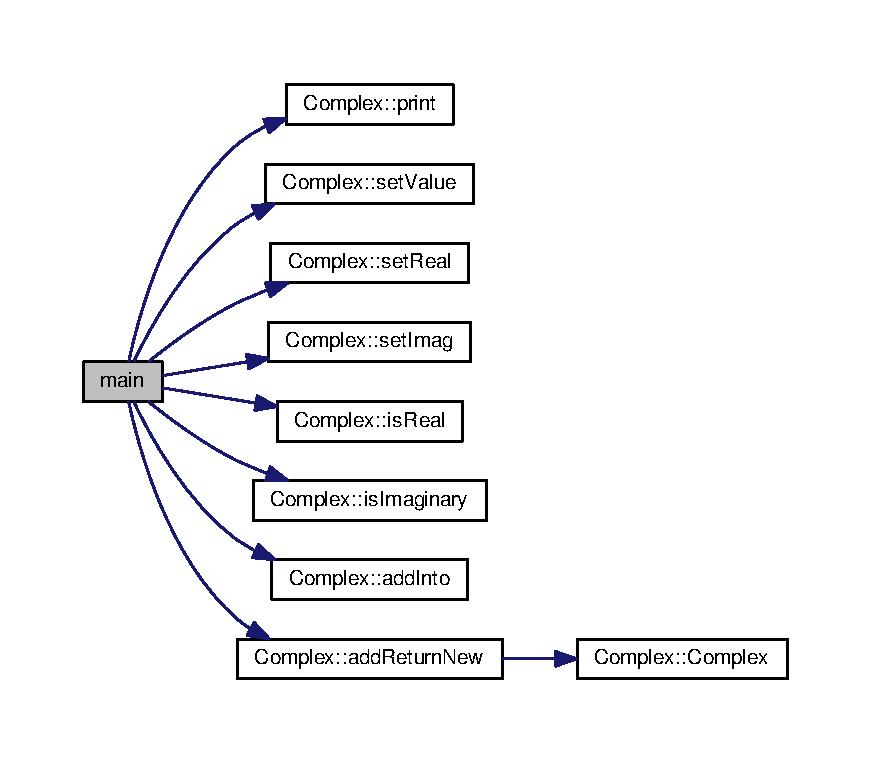
\includegraphics[width=350pt]{Cmain_8cpp_ae66f6b31b5ad750f1fe042a706a4e3d4_cgraph}
\end{center}
\end{figure}



\hypertarget{Complex_8cpp}{}\section{Complex.\+cpp File Reference}
\label{Complex_8cpp}\index{Complex.\+cpp@{Complex.\+cpp}}
{\ttfamily \#include $<$iostream$>$}\\*
{\ttfamily \#include \char`\"{}Complex.\+h\char`\"{}}\\*
Include dependency graph for Complex.\+cpp\+:
\nopagebreak
\begin{figure}[H]
\begin{center}
\leavevmode
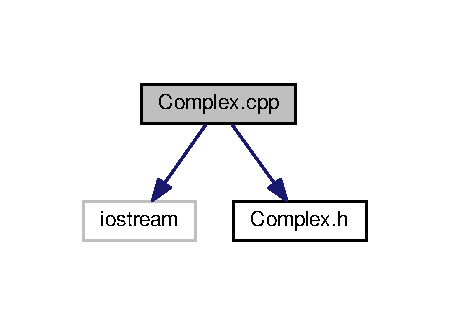
\includegraphics[width=216pt]{Complex_8cpp__incl}
\end{center}
\end{figure}

\hypertarget{Complex_8h}{}\section{Complex.\+h File Reference}
\label{Complex_8h}\index{Complex.\+h@{Complex.\+h}}
This graph shows which files directly or indirectly include this file\+:
\nopagebreak
\begin{figure}[H]
\begin{center}
\leavevmode
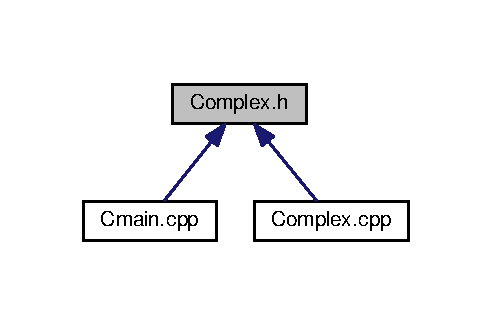
\includegraphics[width=236pt]{Complex_8h__dep__incl}
\end{center}
\end{figure}
\subsection*{Classes}
\begin{DoxyCompactItemize}
\item 
class \hyperlink{classComplex}{Complex}
\end{DoxyCompactItemize}

%--- End generated contents ---

% Index
\backmatter
\newpage
\phantomsection
\clearemptydoublepage
\addcontentsline{toc}{chapter}{Index}
\printindex

\end{document}
